% !TEX root = ./cvl.tex
\section{Experimental Results}
\label{sec:experimental}

\martin{Compare experimental results with theory e.g. expected approximation guarantee, number of constraints, number of records per constraint etc.}

In this section, we present experimental results with our implementation of CVL. Our experiments have the following goals:

\begin{itemize}

\item Evaluate the performance and solution quality of CVL generalizations with a variety of real-world datasets, including point data as well as complex shapes such as polygons and line strings. 

\item Analyze the performance and solution quality of CVL generalizations produced under the proximity and visibility constraints presented in Section~\ref{sec:cvl:language} by both the SGA as well as the LPGA solvers of Section~\ref{sec:algorithms}.

\item Observe how the performance of CVL with different constraints and solvers scales with the number of objects in the geospatial dataset.

\end{itemize}

We start by presenting our experimental setup (Section~\ref{sec:exp:setup}), and then show results for both point data (Section~\ref{sec:exp:points}) and complex shapes (Section~\ref{sec:exp:complex:shapes}). Each result section discusses performance, quality, and scalability. 


\subsection{Experimental Setup}
\label{sec:exp:setup}

\minisec{Datasets}
We have tested CVL using four real-world datasets with the biggest one containing 23 million points and one synthetic dataset containing 30 million points. We list all datasets in Table~\ref{tab:datasets}. 

We have used three point datasets. The airports dataset is from Openflights~\footnote{\texttt{http://openflights.org/data.html}} and contains 7411 airports (points). The tourism dataset contains 500 thousand points representing tourist attractions worldwide from the OpenStreetMap database~\footnote{\texttt{http://www.openstreetmap.org/}}. The fractal dataset (synthetic) was created by iteratively copying and displacing points from the tourism dataset within a 10km radius until 30 million records were reached.

We have used two line segment datasets. The US rivers/streams dataset contains roughly 4 thousand rivers and roughly 27 thousand streams in the United States derived from the OpenStreetMap database. Records with identical name attributes have been merged into one. In the original dataset, most rivers are represented by multiple records, which is unfortunate in a filtering situation (either show the waterway completely or not at all). 

We have used a single polygon dataset, the area information dataset~\footnote{\texttt{http://internet.miljoeportal.dk/}} from The Danish Natural Environment Portal, published by the Danish government. This dataset contains 30 thousand high-fidelity administrative protection zone polygons, and ranging from small polygons the size of buildings to large polygons the size of entire regions. The biggest polygon is described by more than 36 thousand points.

\begin{table}[htdp]
\caption{Datasets used in experiments}
\label{tab:datasets}
\begin{center}
\begin{tabular}{|c|c|c|c|c|}
\hline
\textbf{Origin} & \textbf{Dataset} & \textbf{Type} & \textbf{Records} & \textbf{Points} \\
\hline
Real & Airports & Points & $7K$ & $7K$ \\
Real & Tourism & Points & $500K$ & $500K$ \\
Synthetic & Fractal & Points & $30M$ & $30M$ \\
Real & US rivers & Line segments & $4K$ & $2M$ \\
Real & US rivers/streams & Line segments & $30K$ & $6M$ \\
Real & Proctection zones & Polygons & $30K$ & $9M$ \\
\hline
\end{tabular}
\end{center}
\label{default}
\end{table}%


\minisec{Hardware, Software, and Methods}
The machine used for testing was an Amazon EC2 instance with 17GB RAM, 2 x Intel(R) Xeon(R) CPU E5-2665 0 @ 2.40GHz and 20MB Cache, running Amazon Linux 3.4.48-45.46.amzn1.x86\_64\footnote{An image of the instance we used for testing is available through Amazon EC2 as an AMI. The image contains the exact database used for testing, with all tables preloaded}.

The database used for testing was PostgreSQL 9.2.4 with PostGIS  2.0 built against the following libraries: GDAL 1.9.2 and GEOS 3.3.8. For the LP solver we integrated the database with the convex optimization library CVXOPT version 1.1.6~\cite{cvxopt}. We installed Python language bindings in the database against Python 2.6.8.

We ran each test three times on this installation, taking averages. We observed that measurements were very stable, with negligible difference in compute time between runs.

PostgreSQL always uses a single core to compute a transaction. Because the generalization process in CVL runs as a single long transaction, each job in CVL runs on a single core. A future direction would be to investigate parallel execution of CVL queries using a different language runtime such as a parallel database or a MapReduce environment.

When testing the scalability of CVL using point and datasets we used a line sweep approach for increasing the size of a dataset: We ordered records by minimum x-coordinate, and used prefixes of this order to increase dataset set. The advantage of this approach over random sampling is that the spatial density of records is better preserved.

\minisec{Average optimality ratio}
In our approach we solve the multi-scale filtering problem as a series of single-scale filtering problems. Ideally we would like to compare the objective value of our multi-scale solution to a lower bound or an optimal solution to the multi-scale filtering problem. However, due to the scale of the multi-scale problem, we have not developed a method for computing a lower bound or an optimal solution.

In order to get an indication of solution quality, we have instead compared the solutions to the single-scale filtering problems to the lower bounds coming from solving the LP-relaxation of the integer program for the single-scale filtering problem. The numbers we present in Table~\ref{tab:points:overview} and Table~\ref{} are obtained by computing the average ratio between our solution value and the corresponding lower bound for each zoom level. 

\subsection{Point Data}
\label{sec:exp:points}

In this section, we present experimental results with point datasets, namely the Openflight airports and Tourist attractions datasets. After a quick overview of the results, we then discuss performance and quality breakdowns for CVL and then proceed to analyze CVL's scalability behavior. Even though we experimented with all combinations of solvers (SGA / LPGA) and constraints (visibility / proximity / combined), we show only representative results for brevity. Results for the combined visibility and proximity constraints exhibited the same performance trends as of the most expensive of the two constraints. All other results followed similar trends as the ones explored below. 

An overview of running times and solution qualities for the point datasets are shown in Table~\ref{tab:points:overview}. In Section~\ref{sec:algorithms:sga} we wrote that SGA is optimal for disjoint conflict sets. This is confirmed by the entries for visibility + SGA in the table. For the point datasets we used for testing, the LPGA algorithm is also optimal or within $3\%$ of the optimum when combined with the visibility constraint. Recall that the approximation guarantee of LPGA is $f$, see Section~\ref{sec:algorithms:lpga}.

\begin{table}[htdp]
\caption{Results for CVL on point datasets group by constraint}
\begin{center}
\begin{tabular}{|c|c|c|c|c|}
\hline
\textbf{Dataset} & \textbf{Constraint} & \textbf{Solver} & \textbf{Time} & \textbf{Avg. opt. ratio}\\ 
\hline
Airports (7K) & Visibility & SGA & 7s & 1.0 \\
Airports (7K) & Visibility & LPGA & 7s & 1.03 \\
Tourism (500K) & Visibility & SGA & 6m 9s & 1.0 \\
Tourism (500K) & Visibility & LPGA & 13m 35s & 1.0 \\
\hline
Airports (7K)  & Proximity  & SGA & 3s & 1.18 \\
Airports (7K)  & Proximity & LPGA & 7s s & 1.22 \\
Tourism (500K) & Proximity & SGA & 7m 17s & 1.21 \\
Tourism (500K) & Proximity & LPGA & 2h 18m & 1.24 \\
\hline
\end{tabular}
\end{center}
\label{tab:points:overview}
\end{table}%

\begin{figure*}[tb]
  \begin{minipage}{0.329\linewidth}
    \centerline{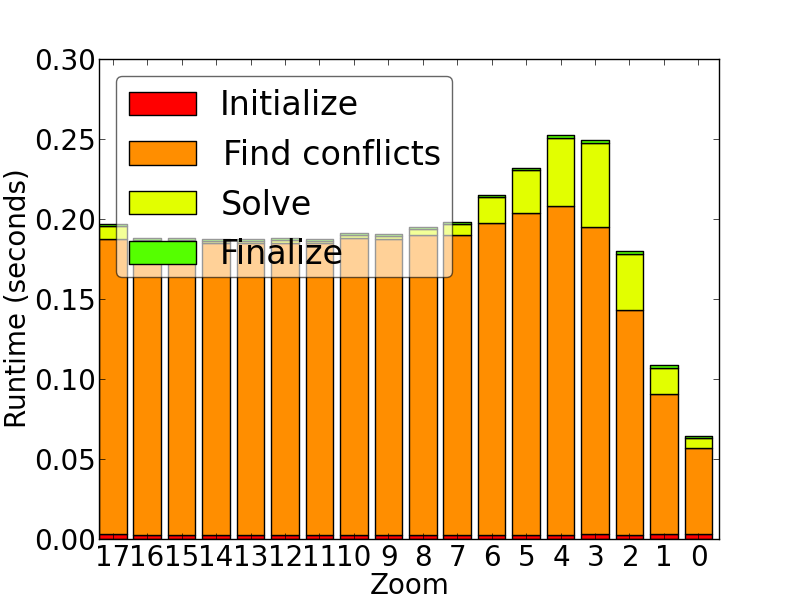
\includegraphics[width=1.0\linewidth]{./figs/prelim_pnt_7k_airports_heuristic_B.png}}
    \centerline{(a) SGA + Proximity}
  \end{minipage} \hfill
  \begin{minipage}{0.329\linewidth}
    \centerline{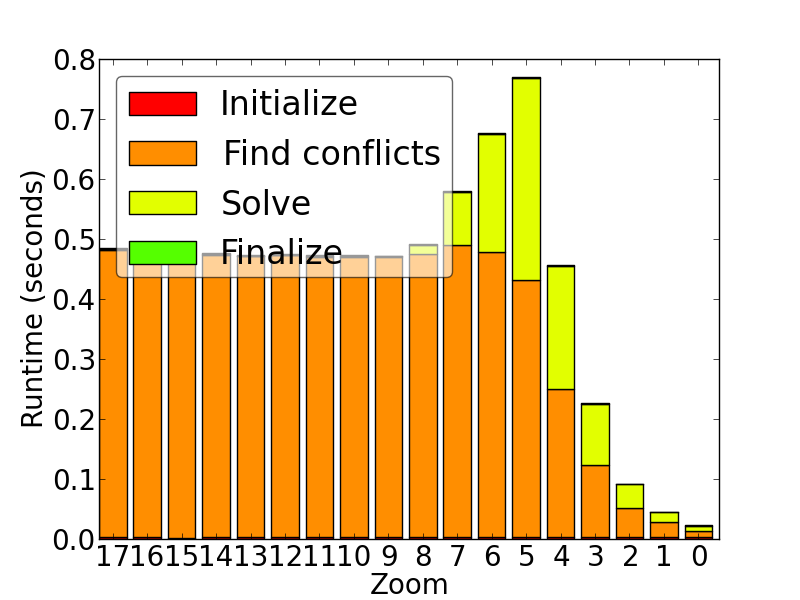
\includegraphics[width=1.0\linewidth]{./figs/prelim_pnt_7k_airports_lp_A.png}}
    \centerline{(b) LPGA + Visibility}
  \end{minipage} \hfill
  \begin{minipage}{0.329\linewidth}
    \centerline{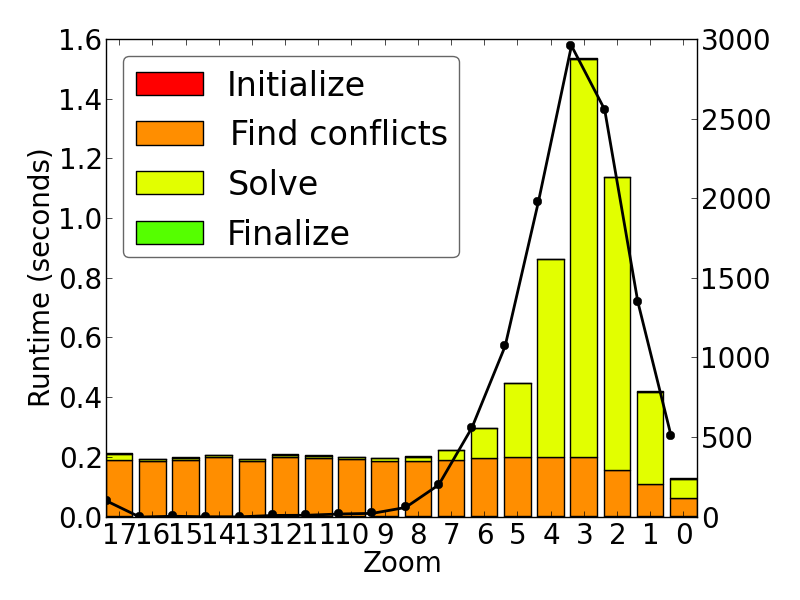
\includegraphics[width=1.0\linewidth]{./figs/prelim_pnt_7k_airports_lp_B.png}}
    \centerline{(c) LPGA + Proximity}
  \end{minipage}
  \vspace{-0ex}
  \caption{Performance breakdown by zoom level, Airport dataset (7K points). Black line indicates number of conflicts} \label{fig:performance:airport}
  \vspace{-2ex}
\end{figure*}

\begin{figure*}[tb]
  \begin{minipage}{0.329\linewidth}
    \centerline{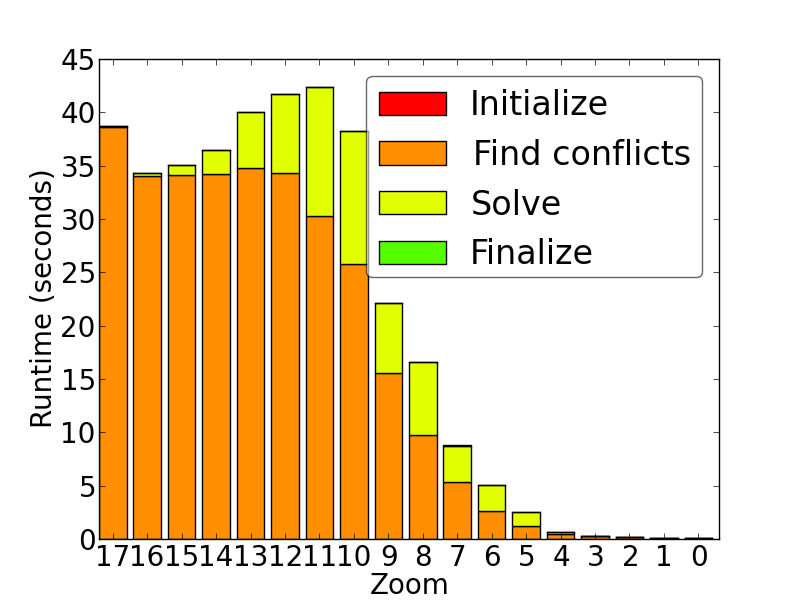
\includegraphics[width=1.0\linewidth]{./figs/prelim_pnt_500k_tourism_heuristic_A.png}}
    \centerline{(a) SGA + Visibility}
  \end{minipage} \hfill
  \begin{minipage}{0.329\linewidth}
    \centerline{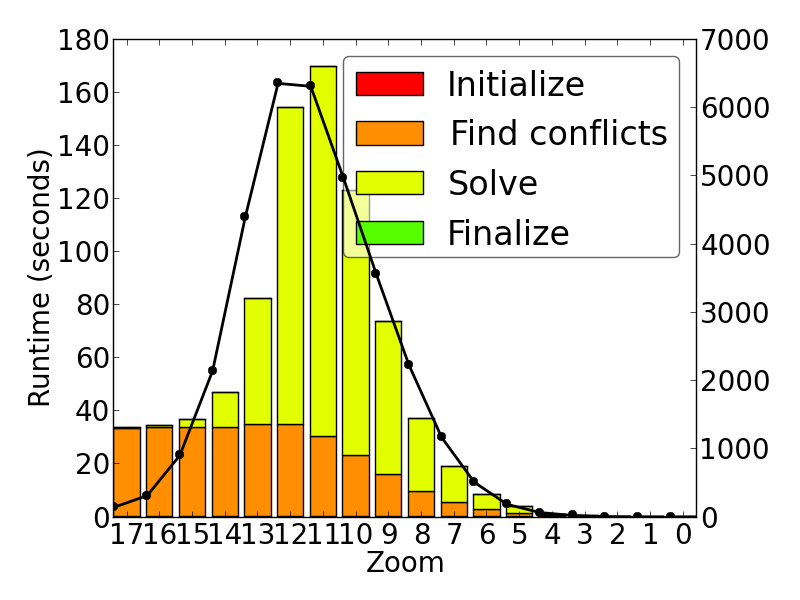
\includegraphics[width=1.0\linewidth]{./figs/prelim_pnt_500k_tourism_lp_A.png}}
    \centerline{(b) LPGA + Visibility}
  \end{minipage} \hfill
  \begin{minipage}{0.329\linewidth}
    \centerline{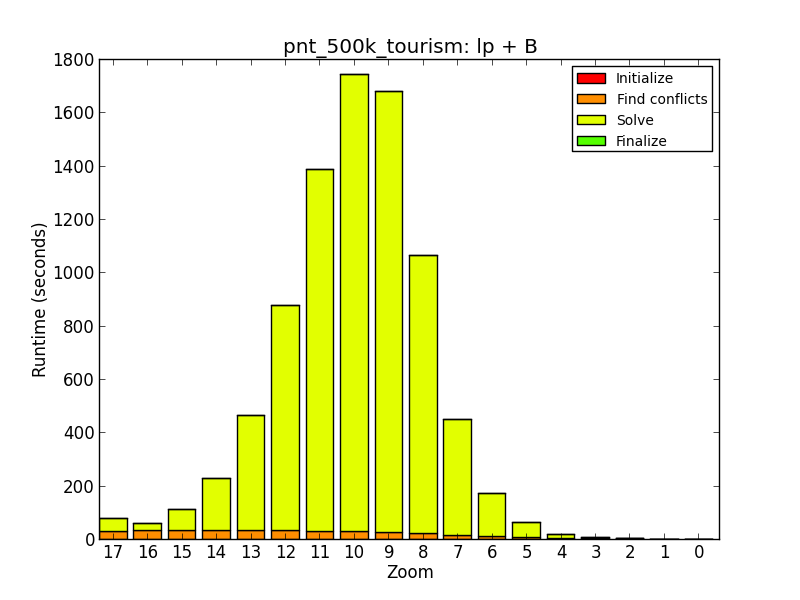
\includegraphics[width=1.0\linewidth]{./figs/prelim_pnt_500k_tourism_lp_B.png}}
    \centerline{(c) LPGA + Proximity}
  \end{minipage}
  \vspace{-0ex}
  \caption{Performance breakdown by zoom level, Tourism dataset (500K points). Black line indicates number of conflicts} \label{fig:performance:tourism}
  \vspace{-2ex}
\end{figure*}

\minisec{Performance breakdown}
 Figure~\ref{fig:performance:airport} shows the performance breakdown per zoom level of executing CVL with the Openflight airports dataset. Note the different y-scales in the graphs. In Parts~(a)-(c), we observe that the time needed to find conflicts is roughly stable until eight zoom levels, then slightly increases, and finally drops sharply for lower zoom levels. The constraints used generate few conflicts at higher zoom levels, given the relatively low density of the airport distribution in space. Nevertheless, even though almost no conflicts are generated, the dataset is still processed, resulting in roughly equal time for finding conflicts and negligible time for solving conflicts per zoom level. 
 
As zoom levels decrease, more conflicts naturally arise, leading initially to increased conflict finding time, as well as conflict solving time. However, as conflicts are solved, records are deleted from the dataset taken as input for the next zoom level. This procedure causes conflict finding time (and eventually total time) to drop significantly for low zoom levels. For SGA under the proximity constraint (Part (a)), total time at zoom level zero is over two times shorter than the initial runtime at zoom level 17; for LPGA under the visibility constraint (Part (b)), the difference in total time reaches over an order of magnitude.  

Conflict solving time does not increase equally for different solvers. SGA exhibits conflict solving time that is consistently smaller than LPGA. Peak total time for SGA under the proximity constraint (Part (a)) is roughly four times shorter than for LPGA (Part (c)). In addition, LPGA is extremely sensitive to the number of conflicts reported by user-defined constraints. From Parts (b) and (c), we can see that LPGA exhibits peak conflict solving time over three times larger for the proximity constraint than for the visibility constraint, since the latter generates far fewer conflicts than the former. The number of conflicts per level is plotted as a black line on the performance breakdown charts.

In terms of quality, the difference between SGA and LPGA is not stark, and depends more on the constraint than on the solver. This can be seen in Table~\ref{tab:points:overview}.

Figure~\ref{fig:performance:tourism} exhibits results with the larger tourism attraction dataset. Since the dataset is denser in space than the airport dataset, conflicts are found and solved at higher zoom levels, resulting in an earlier drop in total time per zoom level. For Parts (a)-(c), total time is uninteresting for zoom levels lower than five. The same cannot be said, however, about peak total time in general, and about conflict solving time in particular.

Parts (a) and (b) compare performance of SGA and LPGA under the visibility constraint. Even though visibility generates a smaller number of conflicts than proximity, peak total time for LPGA is still roughly a factor of four larger than for SGA (see zoom level 11). Note that the difference is completely due to the efficiency of the solver, since the time to find conflicts is essentially the same for both methods. Total time for LPGA rises prohibitively when we employ the proximity constraint, reaching a baffling peak of near half an hour at zoom level 10 (Part (c)). While not shown, total times per zoom level for SGA under the proximity constraint are roughly comparable to the times reported in Part (a) for the visibility constraint using this dataset. SGA's peak total time is slightly above 40 seconds, roughly a factor of 40 smaller than LPGA's.         

While SGA performs significantly better than LPGA, it does not do so at the cost of quality. As discussed in Section~\ref{sec:algorithms:sga}, SGA is optimal for the visibility constraint, since conflict sets are disjoint. For the proximity constraint, TODO

\marcos{Add quality argument above for SGA vs. LPGA for proximity constraint when we get the numbers.}


\minisec{Scalability}

We tested the scalability of CVL for point datasets using the synthetic dataset of 30 million points. The running time of each solver/constraint combination is plotted as a function of dataset size in Figure~\ref{fig:scalability:points}.

We found that SGA scales a lot better than LPGA, which confirms the conclusion we made for the performance breakdown above. We scaled the experiment up to 4 million points, after which the running time became prohibitively large (more than 3 hours) even for SGA. There is a curious fall in running time for SGA with the proximity constraint. We did not gather sufficient data during the scalability experiment to explain this phenomenon. One possible explanation could be that the additional points caused more conflicts, leading to more massive deletion of points during an early stage of the generalization process.

\begin{figure}[htbp]
\begin{center}
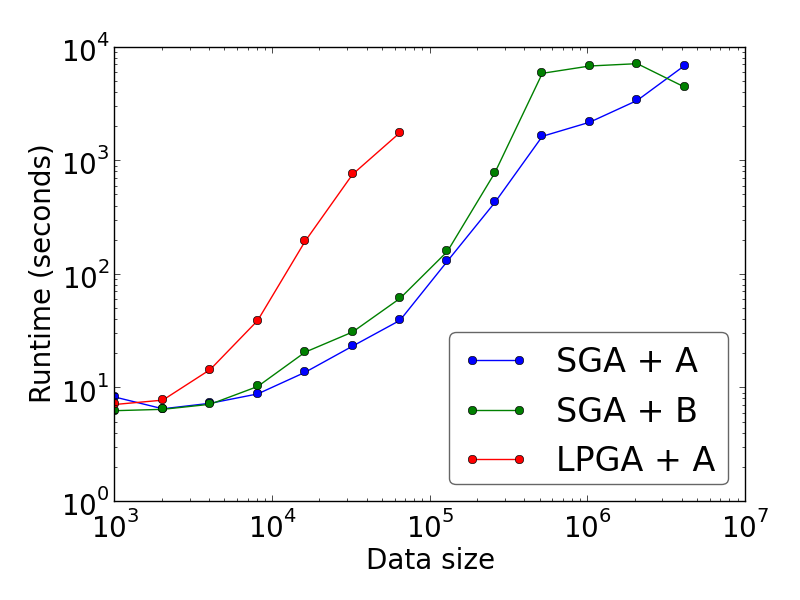
\includegraphics[width=1.0\linewidth]{./figs/scal_pnt_30m_synthetic.png}
\caption{Scalability for point datasets with different algorithms and constraints (visibility=A, proximity=B). SGA has better scalability.}
\label{fig:scalability:points}
\end{center}
\end{figure}

The combination of LPGA + Proximity + Points does not scale. We have excluded these from the test.

\subsection{Complex Shape Data}
\label{sec:exp:complex:shapes}

In Table~\cite{tab:complex:overview} we summarize running times and average optimality ratios for complex shape data. We immediately observe that the average optimality ratio for the visibility constraint is no longer $1.0$ for the SGA solver. This is because the conflict sets are no longer disjoint.

\begin{table}[htdp]
\caption{Results for CVL on complex datasets grouped by constraint}
\begin{center}
\begin{tabular}{|c|c|c|c|c|}
\hline
\textbf{Dataset} & \textbf{Constraint} & \textbf{Solver} & \textbf{Time} & \textbf{Avg. opt. ratio}\\ 
\hline
Rivers (4K) & Visibility & SGA & 1h 32m & 1.36 \\
Rivers (4K) & Visibility & LPGA & 1h 33m & 1.0 \\
Zones (30K) & Visibility & SGA & 13m 38s & 1.20 \\
Zones (30K) & Visibility & LPGA & 32m 15s & 1.14 \\
\hline
Rivers (4K)  & Proximity  & SGA& 1h 11m s & 1.46 \\
Rivers (4K)  & Proximity & LPGA & 1h 31m & 1.11 \\
Zones (30K) & Proximity & SGA & 4h 28m & 1.72 \\
Zones (30K) & Proximity & LPGA & --- & --- \\
\hline
\end{tabular}
\end{center}
\label{tab:complex:overview}
\end{table}%


\minisec{Performance breakdown}

In Figure~\ref{fig:performance:complex} we have selected three performance breakdowns for the two complex datasets. What we see is that, for complex shape datasets, the running time is mostly dominated by the time spent finding conflicts. Finding conflicts operates over the geometric properties of the data, and requires time proportional to the number of points that make up each complex shape. When solving conflicts, the running time is independent of geometric complexity. This causes the running time to be dominated by finding conflicts for complex shape datasets.

The LPGA solver is the exception when there are a lot of conflicts, were it consumes a lot of time. A similar effect was seen for points, indicating that the LPGA solver does not scale well, which is confirmed in our scalability experiments.

\begin{figure*}[tb]
  \begin{minipage}{0.329\linewidth}
    \centerline{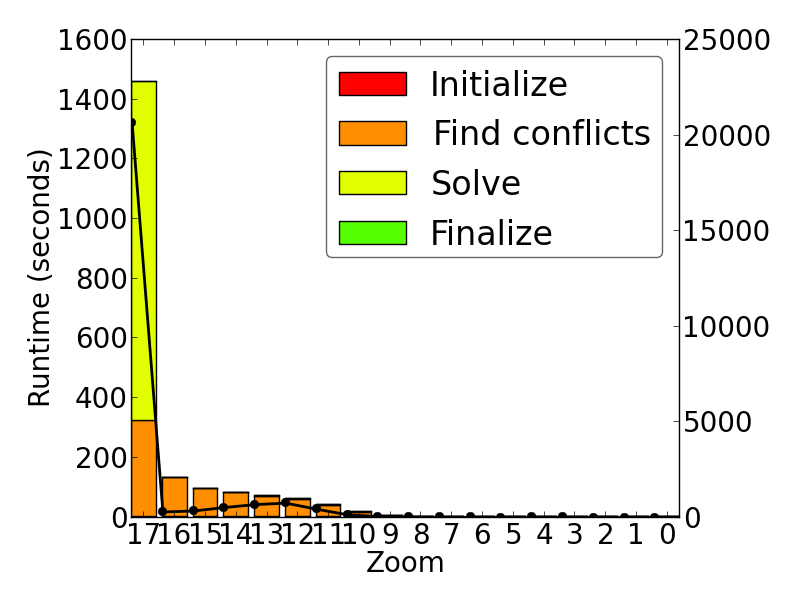
\includegraphics[width=1.0\linewidth]{./figs/prelim_pol_30k_dai_lp_A.png}}
    \centerline{(a) Zones: SGA + Proximity}
  \end{minipage} \hfill
  \begin{minipage}{0.329\linewidth}
    \centerline{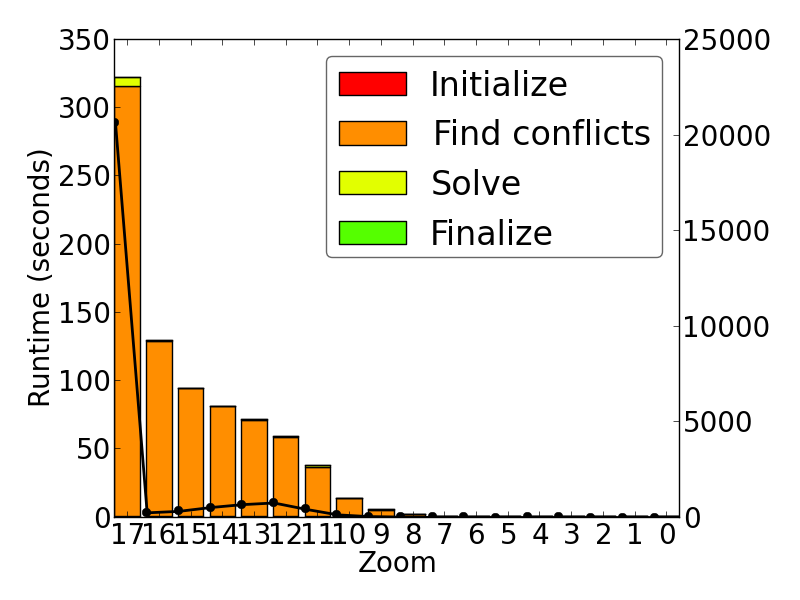
\includegraphics[width=1.0\linewidth]{./figs/prelim_pol_30k_dai_heuristic_A.png}}
    \centerline{(b) Rivers: SGA + Visibility}
  \end{minipage} \hfill
  \begin{minipage}{0.329\linewidth}
    \centerline{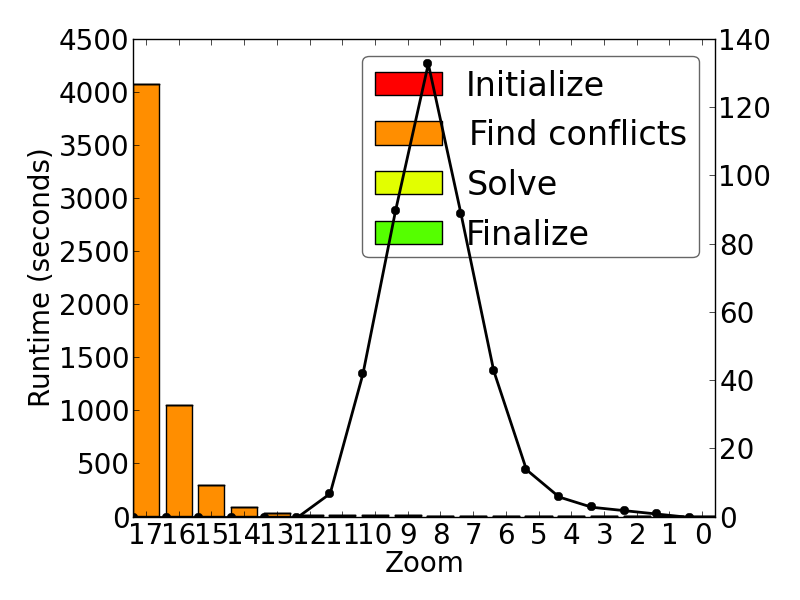
\includegraphics[width=1.0\linewidth]{./figs/prelim_lin_30k_uswaterway_lp_A.png}}
    \centerline{(c) Rivers: LPGA + Visibility}
  \end{minipage}
  \vspace{-0ex}
  \caption{Performance breakdown by zoom level for complex shapes. Running time is most often dominated by finding conflicts. Black line indicates number of conflicts} \label{fig:performance:complex}
  \vspace{-2ex}
\end{figure*}


\minisec{Scalability}

In Figure~\ref{fig:scalability:complex} we show scalability results for complex shape data. Here the scalability depends more on the choice of constraint than the choice of solver. The proximity constraint scales much worse than the visibility constraint. This is because the running time of the distance test used in the proximity constraint is proportional to the product of point counts in the two geometric shapes used in each comparison. Evaluating the visibility depends on the number of tiles that each shape intersects, which depends more on the length or area of each shape. 

While constraints matter more to scalability for complex shapes, the SGA solver scales better than LPGA, which was also the case for our point data.

\begin{figure}[htbp]
\begin{center}
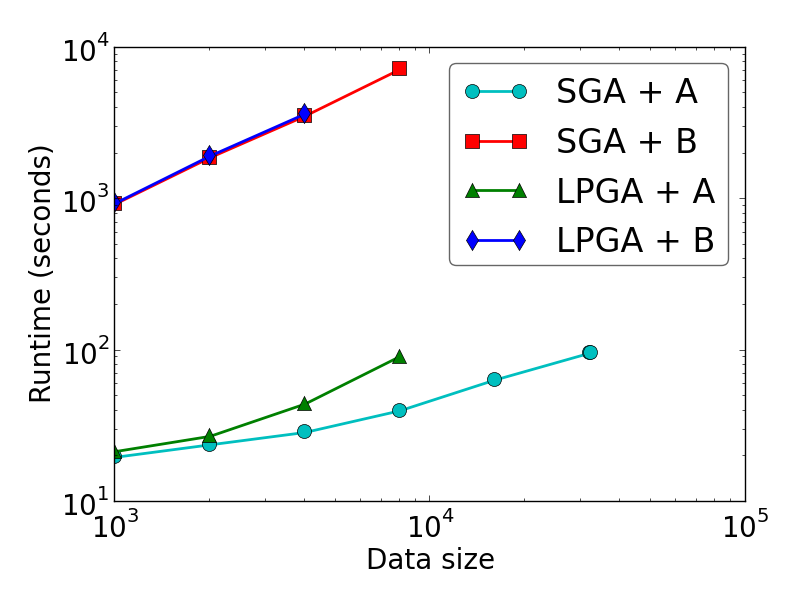
\includegraphics[width=1.0\linewidth]{./figs/scal_lin_30k_uswaterway.png}
\caption{Scalability for US waterway datasets using different algorithms and constraints (visibility=A, proximity=B). SGA has better scalability.}
\label{fig:scalability:complex}
\end{center}
\end{figure}

